\documentclass[10pt,conference,compsocconf]{IEEEtran}

\usepackage[hyphen]{url}
\usepackage{hyperref}
\usepackage{graphicx}	% For figure environment
\usepackage{breakurl}


\begin{document}
\title{The \textit{place} (physical and conceptual) of advertising in video game magazines}
\author{
  Hugo Hueber (\textit{Cybersecurity, MSc}) \& Florine Réau (\textit{Data Science, MSc})\\
  \textit{Supervised by}\\Yannick Rochat (\textit{UNIL GameLab, PhD}) \& Magalie Vetter (\textit{PSL - École nationale des chartes, MSc})
}

\maketitle

\begin{abstract}
  %\textbf{TODO} Short  description  of  the  whole  paper,  to  help  the reader decide whether to read it. State the problem, say why it is an interesting problem, say what your solution achieves, say whaat follows from your solution.
  The video game press has undergone many changes since the 1980s–and the business of advertising has followed. We want to study the evolution of advertising through this specialized press. We use Selective Search to identify areas of interest in a magazine, set up a pre-trained Region-Based Convolutional Networks (R-CNN) then specialized on \textit{Génération 4} magazine to recognize and classify different parts of a magazine, in particular the advertisements. Our model obtains consistent results, and could further be deployed to produce specialized models per magazine and per time period.
\end{abstract}

\section{Introduction}
% \textbf{TODO} \textit{Describe your problem and state your contributions. Why the problem is interesting, is it still unsolved or are current solutions unsatisfactory. Compare with state-of-the-art if any.}
The first French magazine specialized in video games was published in 1982. After a golden age in the 1990s, a reduction in the magazines supply was observed in the 2000s when media started publishing online, with further diversification seen in 2012\cite{claireblandin2018}. Based on this challenging history, we want to analyze the evolution of advertising in the specialized press, as well as the techniques used to advertise. We want to apply image recognition and machine learning techniques to determine the place - position as well as aim - of advertising in this very press over time. To our knowledge, few research on this particular subject has been carried out\footnote{This was discussed with our supervisors. We only have \url{https://www.ludov.ca/fr/documentation/evolution-de-la-publicite}}.

The technical resolution of text classification is an existing field, but nothing specific has been found for the classification of magazine parts\footnote{Some research has been pursued at Montreal, without publication.}, particularly techniques for classifying the pages of paper magazines, in order to be able to differentiate between "advertising" and "non-advertising" pages\footnotemark[1]. Parallels with learning on comics or books could however be done.

\section{Analysis of the available corpus and focus on selected examples}
% \textbf{TODO} 
On www.abandonware-magazines.org, there are 12'328 magazines listed\footnote{https://abandonware-magazines.org/liste.php?tri=identifiant}. We identified two problems. The first one is that not all magazines are correctly scanned: some of the scans are of low quality, incomplete, or simply missing. The second is that these magazines have different mock-ups, also evolving separately over time. Therefore, the changing diversity of magazines would be too broad to study. We thus need to focus on a few selected samples.

If we take \textit{Tilt}, \textit{Joystick Hebdo}, \textit{Joystick} and \textit{Génération 4}, over the years 1988-1998, without the special series, we obtain 326 digitized copies. With an average of 120 pages per issue\footnote{The selected publications are large editions.}, we have about 39'000 pages to study.

\section{Models and methods}
We considered that the detection of magazine pages could be achieved by following a pattern recognition: summary pages always respect a kind of hierarchy, article pages generally have a lot of text, advertising pages often have a main image, etc. So we had to think about crossing the magazines to check these patterns.
%\textbf{TODO} Model: mathematical model or structure ; Methods: algorithms used.
%\begin{enumerate}
%\item Layout the model used
%\item Describe algorithms used, with details (hyperparameters) and preprocessing (e.g. normalizing)
%\item Explain how materials were prepared OK
%\item Describe research protocol
%\item Explain how mesurements were made and what calculations were performed
%\end{enumerate}

\subsection{Model selection}
%\textbf{TODO} \textit{"We were recommended to look at the CNNs", "it turns out that the Faster R-CNN is not bad."}
\begin{figure}[htbp]
    \centering
    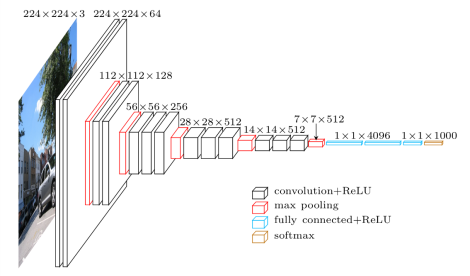
\includegraphics[width=\columnwidth]{vgg16.png}
    \caption{VGG16 architecture\footnote{Taken from \url{http://www.cs.toronto.edu/~frossard/post/vgg16/}.}}
    \vspace{-3mm}
    \label{fig:vgg}
\end{figure}

Our model is based on the Region-based Convolutional Network (R-CNN)\cite{7112511}. We have chosen this model on the one hand on the advice of our tutors, on the other hand because they have a reputation for being particularly effective in image recognition\footnote{\url{https://www.quora.com/What-is-the-difference-between-CNN-and-RNN}}.

Many alternatives and evolutions of R-CNN exist and continue to appear in the domain\cite{rohithgandhi2018}. We have chosen to stick with R-CNN, because of the apparent ease of implementation. A further work will have to be done to compare the other models.

It is to be considered that learning for image recognition is something that is regularly done. We have thus made the choice to use transfer learning\cite{prakashjay2017}, and to reuse existing training. For this particular problem, we went with VGG16\cite{simonyan2014deep}, and loaded pretrained weights from the ImageNet dataset.

We froze the first layers (namely, pooling and convolution), and only modified the fully connected layers, that we dynamically defined regarding the number of classes. For the loss function, we are using categorical cross-entropy\footnote{\url{https://gombru.github.io/2018/05/23/cross_entropy_loss/}}, because our model should output probabilities over the set of all classes.

\subsection{Data cleaning and processing}
% \textbf{TODO} \textit{"How we selected our copies" + "How we selected our classes" + "We made a script to convert XML into a usable format".}


\subsubsection{"Data concierge"}

As mentioned above, the data come from the website \url{https://abandonware-magazines.org}. The data consist only of scans in image form, without integrated text\footnote{\url{https://en.wikipedia.org/wiki/Optical_character_recognition}}. The labelling of the images had to be done manually, with the LabelImg\footnote{\url{https://github.com/tzutalin/labelImg}} software.

Due to a lack of continuity in the data on the one hand\footnote{Some magazines are not complete, some series are not complete, some magazines are not freely available to download, etc.}, and a lack of time to label all magazines on the other hand, we decided to focus on Gen4 magazine. We thus obtained 2'012 pages for our work.

Part of Magalie Vetter's work\footnote{This project is made for her future Master 2 research thesis entitled "1988-1998: captive press? Presence and impact of advertisers in the French videogame press" (working title). In particular, she wishes to train a neural network to automatically detect the presence and location of advertising in this period's various magazines.} consisted in selecting the granularity of the classes. The latter were therefore chosen in agreement with her project manager. A future study will make it possible to refine the choice of these classes.

\subsubsection{Area of interests}
For each image, the principle is as follows: first we perform the image analysis to identify areas of interest via selective search\cite{ss} implemented in OpenCV. We then iterate on the first N results to classify them with our model, according to a predefined threshold.

\begin{figure}[htbp]
    \centering
    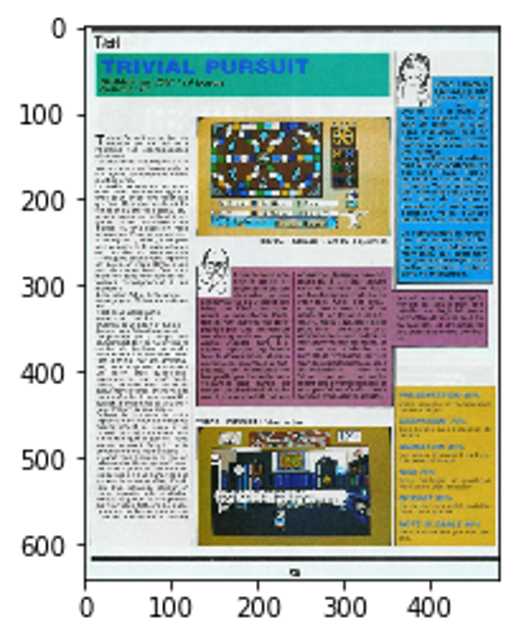
\includegraphics[width=0.5\columnwidth]{example_page.png}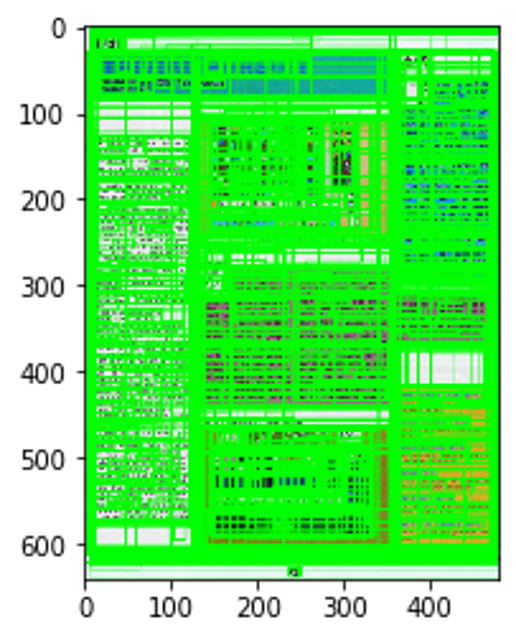
\includegraphics[width=0.5\columnwidth]{example_page_ss.png}
    \caption{Left: Page example; Right: Area of interests using Selective Search.}
    \vspace{-3mm}
    \label{fig:pages-example}
\end{figure}

A significant amount of these areas are of no interest. However, we can keep some of them to be able to make "counter-examples" and classify the "background" zones.

\subsection{Hyperparameters, preprocessing, and other long words}
%\textbf{TODO} \textit{"How do we tuned our model to be particularly effective on the problem at hand."}
\subsubsection{Preprocessing}
The data is not annotated on the website, we have to do it by hand. We then receive the annotations as XML files in PASCAL VOC format, for images in the JPEG format. In order to adapt them to the model, we have created two classes, one to process the annotations and convert them to the right format for our model, while saving them to disk for easy access, the other to process the images and build the corresponding extended dataset - again, with the possibility to store them on disk.

\subsubsection{Hyperparameters tuning}
We train multiple models on three parameters, namely the optimizer (Adam or Nadam\footnote{\url{https://keras.io/optimizers/}}), the learning rate and the batch size (16, 32, 64, 128, dynamic). The learning rate was tested between $0.001$ and $0.01$, while the dynamic batch size was basically a function of the samples number. We tried to optimize the accuracy and reduce the loss.

\begin{table}[]
\centering
\begin{tabular}{|c|c||c|c|c|c|}
\hline
\textbf{LR (best)} & \textbf{Batch size} & \textbf{Loss} & \textbf{Val loss} & \textbf{Acc} & \textbf{Val acc} \\ \hline\hline
0.004&16&7.8226&8.2037&0.5147&0.4910\\ \hline
0.002&32&7.2733&8.3210&0.5488&0.4838\\ \hline
0.003&64&7.5174&8.7426&0.5335&0.4576\\ \hline
0.002&128&8.1850&7.6813&0.4922&0.5234\\ \hline
\end{tabular}
\textit{Hyperparameters comparison with Adam optimizer}
\end{table}
\begin{table}[]
\centering
\begin{tabular}{|c|c||c|c|c|c|}
\hline
\textbf{LR (best)} & \textbf{Batch size} & \textbf{Loss} & \textbf{Val loss} & \textbf{Acc} & \textbf{Val acc} \\ \hline\hline
0.002&16&7.7360&7.5656&0.5128&0.5306\\ \hline
0.002&32&7.3539&7.8979&0.5437&0.5100\\ \hline
0.002&64&7.1956&8.7426&0.5536&0.4576\\ \hline
0.002&128&7.3665&7.4924&0.5430&0.5352\\ \hline
\end{tabular}
\textit{Hyperparameters comparison with Nadam optimizer}
\end{table}

The best way to balance accuracy and speed would thus be to use the Napam optimizer, along with a learning rate of 0.002, and 128 samples per batch. We did not use batch\footnote{\url{https://medium.com/analytics-vidhya/train-keras-model-with-large-dataset-batch-training-6b3099fdf366}} at first, but turns out it boosted the learning process, because less cycles are wasted. A further work could add the use of GPU as a basis.

\section{Results}
%\textbf{TODO} \textit{Does the model work? Does the model work well? When confronted with evaluation methods (e.g.), are the results interesting? When confronted with unknown data, are the results interesting?}
%\textbf{TODO} \textit{Compare results. Care should be taken to ensure that the same evaluation methods are used as for the original paper.}
We trained the model on 100 epochs, with 512 pages. We obtain a final accuracy of about 0.5703. The model seems to work and achieve to recognize images, although it is far from perfect. For example, if we use photos from the ground truth, it is obvious that some labels are missing, others are over-represented. The probability analysis given by our model shows us that the final probabilities are rather low (around 0.30), the use of an adapted threshold allows us to obtain more convincing results.

\begin{figure}[tbp]
    \centering
    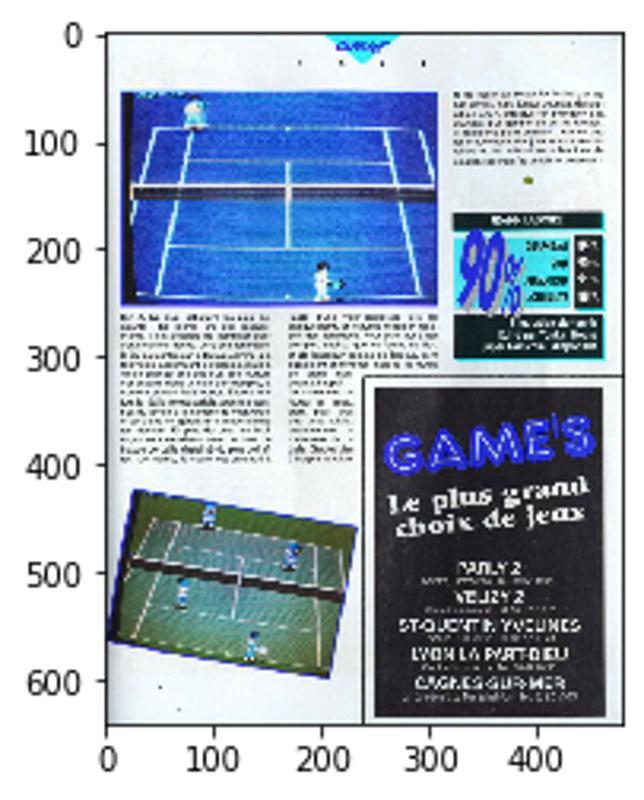
\includegraphics[width=0.5\columnwidth]{page_result.jpg}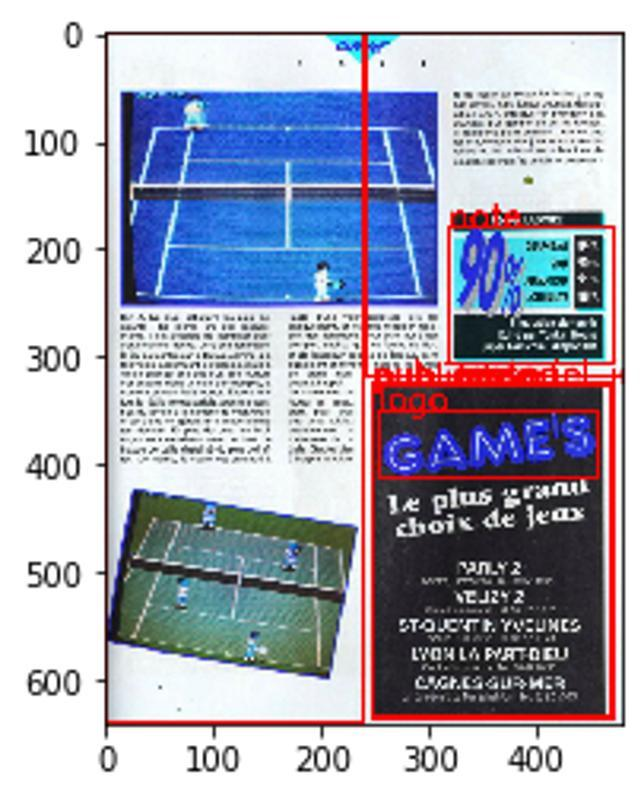
\includegraphics[width=0.5\columnwidth]{page_result_annotated.jpg}
    \caption{Left: Page example; Right: Ground truth.}
    \vspace{-3mm}
    \label{fig:pages-example-2}
\end{figure}
\begin{figure}[tbp]
    \centering
    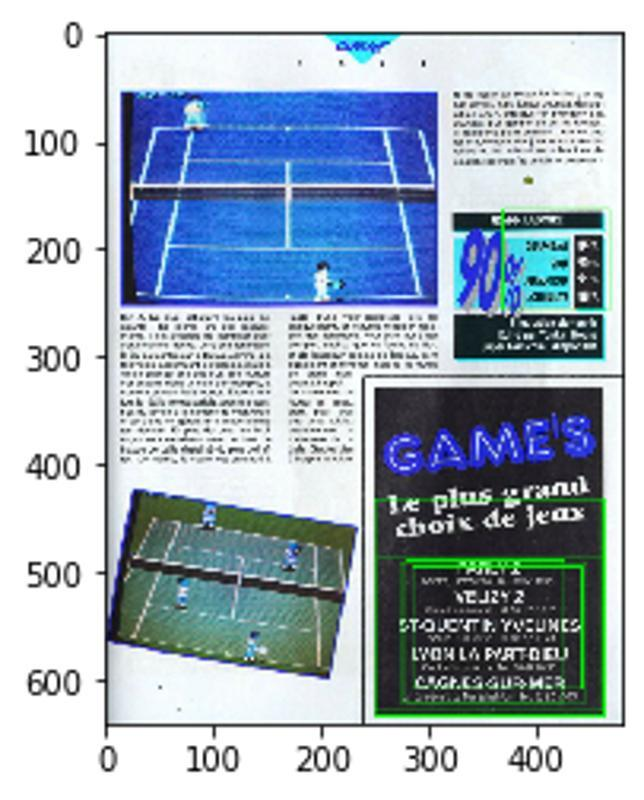
\includegraphics[width=0.5\columnwidth]{page_result_model.jpg}
    \caption{Model labelization, threshold of 0.85.}
    \vspace{-3mm}
    \label{fig:pages-example-2-model}
\end{figure}

When confronted with unknown data, the model responds pretty well. We may want to adapt and specialize it each time we are changing era or magazine.

\section{Further researches}
% \textbf{TODO} \textit{Text recognition for "paid" articles? Probability score based on results?}
The magazines studied are composed of texts and images. In this project, we focus on the differentiation between text and image, one could go further and make a differentiation at the text level (for example between an editorial and an article, or a "normal" article and a sponsored article), and the use of text recognition could be adapted. One could imagine adapting the current pipeline to add a text recognition step, and increase the accuracy of the classification. However, as mentioned above, the text is not integrated into the scan, and pre-processing should also be added in the pipeline. Solutions like Google Vision\footnote{\url{https://cloud.google.com/vision/}} exist.

Also as indicated above, the granularity of the labels would need to be reworked. One solution could be to make thinner labels ("image", "title", etc.), and assign them a "score". The probability of a page being an advertisement could thus be calculated with these then weighed results.

\section*{Acknowledgements}
Thanks Yannick Rochat and Magalie Vetter for supervising our project. Thanks Johan Paratte and Yoann Ponti for their input. Thanks Louis Vialiar and Camille Montemagni for the proofreading and testing.

\bibliographystyle{IEEEtran}
\nocite{*} % Enlever lors des références
\bibliography{literature}

\end{document}

% \begin{figure}[tbp]
%   \centering
%   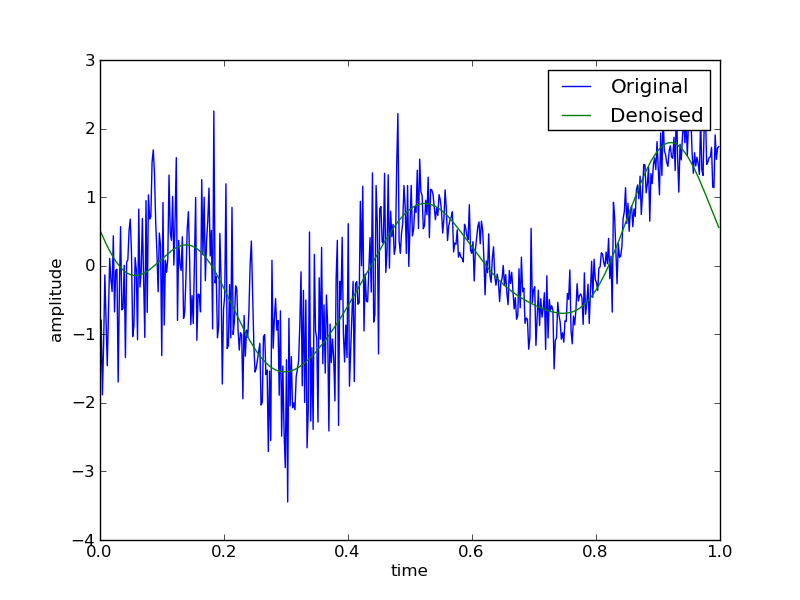
\includegraphics[width=\columnwidth]{denoised_signal_1d}
%   \caption{Signal compression and denoising using the Fourier basis.}
%   \vspace{-3mm}
%   \label{fig:denoise-fourier}
% \end{figure}
% \begin{figure}[htbp]
%   \centering
%   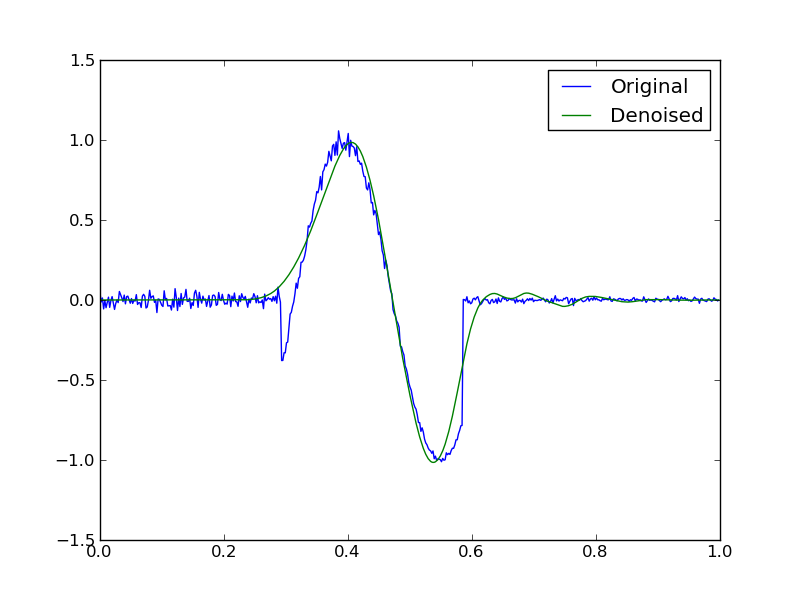
\includegraphics[width=\columnwidth]{local_wdenoised_1d}
%   \vspace{-3mm}
%   \caption{Signal compression and denoising using the Daubechies wavelet basis.}
%   \label{fig:denoise-wavelet}
% \end{figure}